%%%%%%%%%%%%%%%%%%%%%%%%%%%%%%%%%%%%%%%%%
% University Assignment Title Page 
% LaTeX Template
% Version 1.0 (27/12/12)
%
% This template has been downloaded from:
% http://www.LaTeXTemplates.com
%
% Original author:
% WikiBooks (http://en.wikibooks.org/wiki/LaTeX/Title_Creation)
%
% License:
% CC BY-NC-SA 3.0 (http://creativecommons.org/licenses/by-nc-sa/3.0/)
% 
% Modified for COSC480/490 by:
% Lech Szymanski (8/3/18)

\documentclass[12pt]{article}
\usepackage[draft]{cosc4x0style}
\usepackage{biblatex}
\addbibresource{refs.bib}

% To compile the final version of the report (which will remove all the todo content)
%\usepackage{cosc4x0style}

% Specify project code 480 or 490
\papercode{480}

% Your project title
\title{An Exploration of the Common Vulnerability Scoring System}

% Your name
\author{Jake \textsc{Norton}}
\studentid{5695756}

% Names of your supervisors, separated by line break '\\'
\supervisors{
  Dr. David \textsc{Eyers} \\
  Dr. Veronica \textsc{Liesaputra}
}

% Date, change the \today to a set date if you want to be precise
\reportdate{\today}

\begin{document}


\maketitle

\begin{abstract}

	The Common Vulnerability Scoring System(CVSS) is a system designed to produce scores for software
	vulnerabilities. Such a system is needed in order to triage the sheer number of new
	vulnerabilities being released every year. We cannot keep up with the amount of CVSS scores that
	need to be produced, as such we need a way to generate them. There is precedent to using machine
	learning, specifically in more recent times, large language models(LLMS) to accurately predict
	these CVSS scores. However, there is a general focus on only using the National Vulnerability
	Database, it would be ideal if there was more than one source for the ratings, not only for cross
	validation, but also for an increase in data. Before we use any extra data sources, it will be
	interesting to do a comparison between the different sources, to see if we can get an estimate
	accuracy for each of the metrics within the scoring system. Additionally we should know how good
	of a system CVSS is and whether or not there are better alternatives. Unfortunately CVSS is a
	flawed metric, hopefully once 4.0 begins to be used commonly that will solve some of these issues.
	However, the ability to predict a metric based on a short text description is still useful and a
	focus on the interpretability of such a system remains important.

\end{abstract}

\begin{figure}
	\centering
	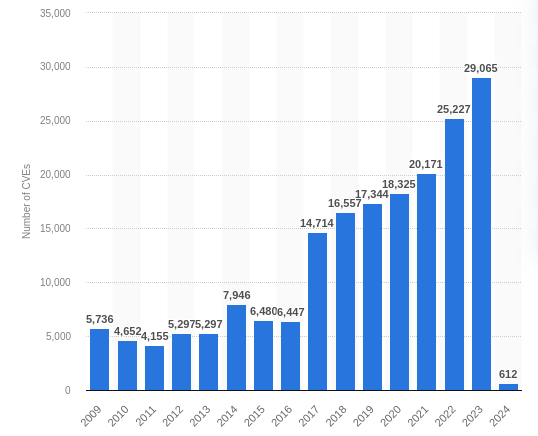
\includegraphics[width=0.5\textwidth]{figures/cve_year.png}
	\caption{\label{fig:cve_year}Number of new CVEs by year}
\end{figure}

\section{Introduction}

Last year there were 29,065 new vulnerabilities. This is a number that is only going
up year on year. Now, we need a way to record these vulnerabilities, and we do that using the common
vulnerabilities and exposure system called CVEs. From these CVEs, CVSS scores can be calculated or
generated. The National Vulnerability Database(NVD) takes the CVEs and enriches them with CVSS data.
They are not the only place to do so, however in terms of research the are often the main or sole
data provider. I explored other options, the main obvious one being MITRE, as they are the main
database for CVEs and they also have a decent chunk of CVEs enriched with CVSS scores. As a
guideline to my investigation between the two databases I used the same method as the paper
\textit{Can the Common Vulnerability Scoring System be Trusted? A Bayesian Analysis}.\cite{bayes}
This paper tries to see how much different data sources agree on the scoring of a CVE, and there by
gaining insight into the potential of a ground truth value. Unfortunately since that paper in 2016,
many of the databases they compared are either unavailable or in archival status. However, following
there method stills allows for insight between the two chosen databases, NVD and MITRE. This
analysis shows that the databases do fundamentally rate CVEs differently. The uncertainty between
the two can therefore be an indicator going forward when analysing generated CVE scores, as it is
likely that the model will also struggle in similar places to where the human evaluators did. In
addition to this analysis, I also looked into the CVSS system itself. There have been many
complaints laid against CVSS\cite{ubiquitous}\cite{improving_cvss}, the main being:

\begin{itemize}
	\item Mathmatical operations on categorical values
	\item No mathmatical basis for the formula
	\item Lack of likelihood
\end{itemize}




\section{Background}

\subsubsection*{Here is an example CVE}
\begin{itemize}
	\item   Unique Identifier: CVE-2024-38526
	\item   Source: GitHub, Inc.
	\item   Published:06/25/2024
	\item   Updated:06/26/2024
	\item   Description: pdoc provides API Documentation for Python Projects. Documentation generated with `pdoc --math` linked to JavaScript files from polyfill.io. The polyfill.io CDN has been sold and now serves malicious code. This issue has been fixed in pdoc 14.5.1.
\end{itemize}

The unique identifier, which is given by one of the CVE numbering authorities, such as GitHub,
Google and many other organizations.[\href{https://www.cve.org/PartnerInformation/ListofPartners}{CVE
			list of partners}] The description is the most important part in our case. This should give some
information about the vulnerability, what can be exploited(device / software component), what it
does if  you have what is the product and then how does the vulnerability affect it. And so we have
PyDoc and this links to the polyfill.io CDN. And so that means that it can also be affected by the
malicious code.

CVSS scoring is a high level way to break up vulnerabilities into different categories so that
organisations can choose which vulnerability to focus on first. CVSS in broken up into 3 distinct sections, base score,
temporal and environmental.

For brevity I will only show the specifics of CVSS 3.1 as this is by far the most commonly used version, even if it is
not the most recent.

\subsubsection*{Base Score}

\begin{itemize}

	\item Attack Vector -> Defines the avenues of attack that the vulnerability is open to. The more open a
	      component is, the higher the score. This can have the values Network, Adjacent, Local and Physical.

	\item Attack Complexity -> How complex the attack is so orchestrate. What are they prerequisites, how much
	      domain knowledge/ background work in necessary, how much effort does the attacker need to invest to
	      succeed. This can have the values Low or High. Low gives a higher base score.

	\item Priviledges Required -> The degree of priviledges the user needs to complete the attack. Generally
	      ranging from None, Low(e.g User level priviledge), High(e.g Administrator). The lower the priviledge
	      the higher the base score.

	\item User Interaction -> If the exploit requires another human user to make the attack possible, E.g
	      clicking a phishing link. This is either None or Required, the score is highest when no user
	      interaction is required.

	\item Scope -> Defines if the attack can bleed into other security scopes. E.g access to one machine gives
	      the ability to elevate privileges on other parts of the system. This can take Unchanged or Changed,
	      the score being highest when a scope change occurs.

	\item Confidentiality Impact -> Detemines what is the impact on the information access / disclosure to the
	      attacker. This can be High, Low or None with High adding the most to the base score.

	\item Integrity Impact -> Refers to the integrity of the information within the component. I.e could the
	      data have been modified by the attacker. This has High, Low or None as categories with High adding the
	      most to the base score.

	\item Availability Impact -> Refers to the impact of the attack on the availability of the component. E.g
	      the attacker taking the component off the network, denying the users access. This can haved High, Low
	      and None with High adding the most to the base score.

\end{itemize}


\section{How to compile \LaTeX{}}

The remaining sections should present what you have done in your project including the results and analysing.  For this document this will be a demonstration of how to use \LaTeX{} in order to create your report.

\LaTeX{} documents are prepared using markup language and need to be compiled to produce pdfs.

The easiest way is to use the \href{https://www.overleaf.com}{Overleaf service} - it's free for private projects.  Create an account and once you login you can create different projects (essentially different documents).  After clicking on "New Project" select "Upload project" and upload the \textit{cosc4x0report.zip} file where this pdf came from.  The template will open on the website and you'll be able to edit the report in your browser, compile LaTeX to pdf online and have it saved on a remote server.  Later you just download the final pdf and submit as your report.

Alternately, you can install a LaTeX compiler on your machine and compile the .tex file yourself.  On macOS you need to download and install \href{http://www.tug.org/mactex/downloading.html}{MacTeX}.  Then, using a program like \href{http://pages.uoregon.edu/koch/texshop/}{TexShop} (free), or \href{https://www.texpad.com/}{Texpad} (awesome, but not free) you can edit and compile a .tex file into the .pdf.

\section{\LaTeX{} markup examples}
\label{sec:examples}

\subsection{Sections}

Use section and subsection commands to organise your document. \LaTeX{} handles all the formatting and numbering automatically. Use ref and label commands for cross-references.

\subsection{Comments}

Comments might be useful during the writing process, as reminders or questions to your supervisor (who should get a chance to comment on your report).  Comments can be added to the margins of the document using the \todo{Here's a comment in the margin!} \verb$\todo{}$ command, as shown in the example on the right. You can also add inline comments too:

\todo[inline, color=green!40]{This is an inline comment.}

\subsection{Tables and Figures}

Use the table and tabular commands for basic tables --- see Table~\ref{tab:widgets}, for example. You can include a figure (JPEG, PNG or PDF) with the \verb$\includegraphics$ command as in the code for Figure~\ref{fig:frog} below.

% Commands to include a figure:
\begin{figure}
	\centering
	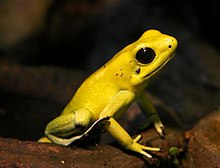
\includegraphics[width=0.5\textwidth]{figures/frog.jpg}
	\caption{\label{fig:frog}This is a figure caption.}
\end{figure}

\begin{table}
	\centering
	\begin{tabular}{l|r}
		Item    & Quantity \\\hline
		Widgets & 42       \\
		Gadgets & 13
	\end{tabular}
	\caption{\label{tab:widgets}An example table.}
\end{table}

\subsection{Mathematics}

\LaTeX{} is great at typesetting mathematics. Let $X_1, X_2, \ldots, X_n$ be a sequence of independent and identically distributed random variables with $\text{E}[X_i] = \mu$ and $\text{Var}[X_i] = \sigma^2 < \infty$, and let
$$S_n = \frac{X_1 + X_2 + \cdots + X_n}{n}
	= \frac{1}{n}\sum_{i}^{n} X_i$$
denote their mean. Then as $n$ approaches infinity, the random variables $\sqrt{n}(S_n - \mu)$ converge in distribution to a normal $\mathcal{N}(0, \sigma^2)$.

\subsection{Lists}

You can make lists with automatic numbering \dots

\begin{enumerate}
	\item Like this,
	\item and like this.
\end{enumerate}
\dots or bullet points \dots
\begin{itemize}
	\item Like this,
	\item and like this.
\end{itemize}

\section{Conclusion}

Concluding remarks.  Send the pdf (not the \verb$*.tex$ file) to your supervisor for comments (as early as possible).  Don't forget to change the \verb$\usepackage[draft]{cosc4x0style}$ setting to \verb$\usepackage{cosc4x0style}$ to produce the pdf for the final submission.

\printbibliography[title={References}]



% Activate the appendix
% from now on sections are numerated with capital letters
\appendix

\renewcommand{\thesection}{Appendix \Alph{section}}

\section{Some extra things}

If you have anything more to add such as:
\begin{itemize}
	\item not essential details - things that might be too much for first time reading, or could be distracting from the main points...but are still important for reproducibility or deeper understanding
	\item work that was done in the project but doesn't go with the
\end{itemize}

\section{Aims and Objectives}

Your last appendix include your original Aims and Objectives.  If the original aims and objectives have changed, specify the original and revised aims and objectives in separate sections.  If you used the \LaTeX{} template provided for your Aims and objectives document, just copy the \verb$\paragraph{Aims}$ and \verb$\paragraph{Objectives}$ sections and paste them here.

\subsection*{Original}

\paragraph{Aims}
Here you are describing the term goal of the project.  What do you want to achieve by the end?  What is the ultimate goal of this work?  For example, the primary aim of this document is to have students produce suitable aims and objectives for their COSC480/490 project.  While the aims and objectives documents is not an assessed deliverable, a clear definition of what is to be done, and a bit of planning of how it is to be accomplished is paramount to the project's success.  It is important to establish the scope of the project.

\paragraph{Objectives}
Objectives list the milestones that you need to achieve in order to achieve the projects aim(s).  It's a rough plan for what needs to happen in what order.  It's best to list the objective in bullet point form.  For many projects the structure to these objective might follow the following pattern (objective names are just examples -- you can have different objective names):
\begin{itemize}[noitemsep]
	\item background reading; going through the literature; learning about the research field;
	\item setting up of some kind of system for the project; getting the environment for experiments working;
	\item conducting preliminary experiments; implementation of a basic/simple approach; ; producing base case results ;
	\item trying method 1; recording the results;
	\item trying method 2; recording the results.
\end{itemize}

\subsection*{Revised}

\paragraph{Aims}
Here you are describing the term goal of the project.  What do you want to achieve by the end?  What is the ultimate goal of this work?  For example, the primary aim of this document is to have students produce suitable aims and objectives for their COSC480/490 project.  While the aims and objectives documents is not an assessed deliverable, a clear definition of what is to be done, and a bit of planning of how it is to be accomplished is paramount to the project's success.  It is important to establish the scope of the project.

\paragraph{Objectives}
Objectives list the milestones that you need to achieve in order to achieve the projects aim(s).  It's a rough plan for what needs to happen in what order.  It's best to list the objective in bullet point form.  For many projects the structure to these objective might follow the following pattern (objective names are just examples -- you can have different objective names):
\begin{itemize}[noitemsep]
	\item background reading; going through the literature; learning about the research field;
	\item setting up of some kind of system for the project; getting the environment for experiments working;
	\item conducting preliminary experiments; implementation of a basic/simple approach; ; producing base case results ;
	\item trying method 1 (A); recording the results;
	\item trying method 1 (B); recording the results.
\end{itemize}


\end{document}
